% !TEX root = QlockToo.tex
% Kapitelvorlage

\section{Funktionen}
\label{sec:Funktionen}

\begin{multicols}{2}

Neben der Darstellung der Uhrzeit in Worten verfügt die entwickelte Wortuhr über zahlreiche weitere Funktionen. Während einige Funktionen und Modi bzw. Demonstrationsmuster nur über die Software ausgewählt werden können, so besteht für die wichtigsten Funktionen die Möglichkeit, diese über vier Taster, welche sich seitlich am Rahmen befinden, auszuwählen. Die Modi, welche über die Software auf die Uhr übertragen werden können, sind im Kapitel~\ref{sec:Software} beschreiben. Zur Übertragung muss die Uhr über die USB~-~Schnittstelle direkt an einen PC angeschlossen sein. 

 \textbf{Tasterbelegung} Durch Drücken der Taster einzeln oder in Kombination sind die nachfolgenden Funktionen auswählbar.  \\ \\
\textbf{Taster 1} Anzeige der Uhrzeit in Worten.

{
\centering
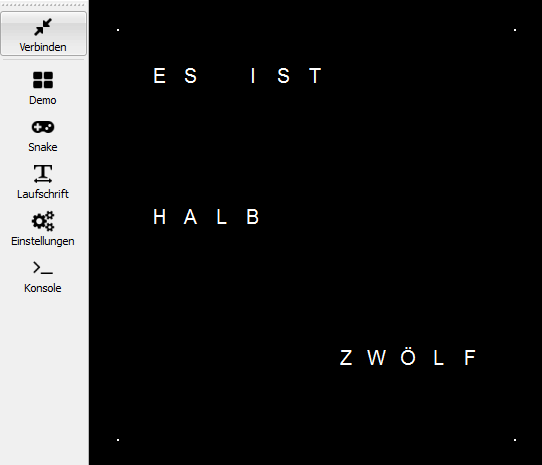
\includegraphics[width=0.8\columnwidth]{Abbildungen/Funktionen/Uhrzeit_01}

}

\textbf{Taster 2} Anzeige der Sekunden.

{
\centering
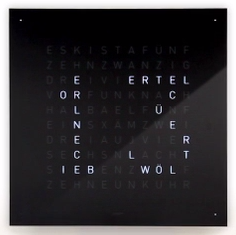
\includegraphics[width=0.8\columnwidth]{Abbildungen/Funktionen/Sekunden_01}

}

\textbf{Taster 3} Anzeige der Raumtemperatur in $^\circ$C.

{
\centering
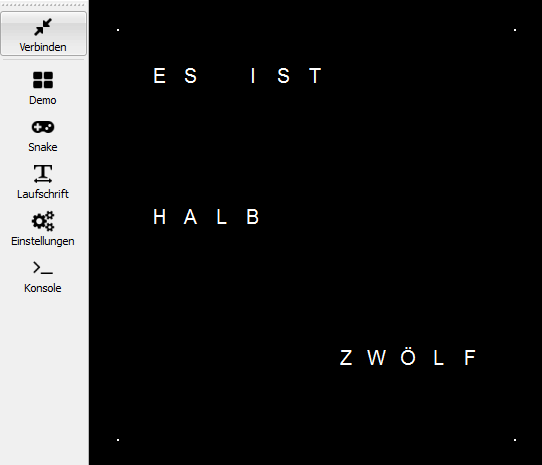
\includegraphics[width=0.8\columnwidth]{Abbildungen/Funktionen/Uhrzeit_01}

}

\textbf{Taster 4} Wird der Taster vier lange gedrückt, so erfolgt die Einstellung der Helligkeit automatisch über einen Helligkeitssensor über der Buchstabenmatrix. Mit Hilfe des Sensors wird die Helligkeit an das Umgebungslicht angepasst. 
Über kurzes Drücken kann die Helligkeit in sieben Stufen manuell ausgewählt werden. Im letzten Modus ist die Uhr aus.

\textbf{Taster 1 \& Taster 2 } Durch das gedrückt halten des ersten Tasters und das gleichzeitige Drücken des zweiten Tasters können zwei Demo Modi ausgewählt werden. Zum Testen der LEDs können alle gleichzeitig eingeschaltet werden. Der zweite Modus ist die Matrix Darstellung, siehe Kapitel~\ref{sec:Software}.

\end{multicols}